\section{Ecuaciones diferenciales Separables}
\begin{itemize}
    \item ED de 1er grado separable: es una ED de 1er grado cuyo lado derecho es un producto de una función en $x$ y una función $y$.
        \[
          \frac{d y}{d x} = f(x)g(y) \qq \text{ o } \qq g(y)dy+f(x)dx=0
        \]
    
    \item Resolución: se coloca cada variable en un lado de la ecuación y se integra respecto a cada variable. Ya con eso eliminamos la derivada, pero debemos resolver para $y$.
        \begin{center}
           \begin{align*}
               \frac{d y}{g(y)} = f(x)dx \qimplies \int \frac{d y}{g(y)} = \int f(x)dx \\ 
               G(y) = F(x) + C \\ 
               \text{ Las dos constantes de integración se pueden combinar en una sola $C = C_2-C_1$  } \\ 
           \end{align*}
        \end{center}
    
    \item Ejemplos: 
        \begin{center}
           \begin{align*}
               \frac{d y}{d x} = y^3x^2e^{x^3+y^4} = (y^3e^{y^4})(x^2e^{x^3}) \qimplies \text{ Separable. } \\ 
               \frac{d y}{d x} = tan(y+x) \qimplies \text{ No es separable. } \\ 
           \end{align*}
        \end{center}
\end{itemize}

\subsection{Ejercicio 1: Resuelva}
Pasos:
\begin{enumerate}
    \item Separe.
    \item Integre.
    \item Resuelva para $y$.
\end{enumerate}
\begin{enumerate}
    \item $\displaystyle \frac{d y}{d x} = -3x^2y^2$ 
        \begin{center}
           \begin{align*}
                \frac{d y}{d x} = -3x^2y^2 \qq \text{ Como un cociente de diferenciales $\frac{d y}{d x} $ }. \\ 
                \frac{d y}{-y^2} = 3x^2dx \qq \text{ Separe. } \\ 
                \int -y^{-2}dy = \int 3x^2dx \qq \text{ Integre. } \\ 
                \frac{1}{y}=x^3+C \qq \text{ Resuelva para $y$ } \\ 
                y = \frac{1}{x^3+C} \\ 
           \end{align*}
        \end{center}
        \begin{itemize}
            \item $\displaystyle \frac{d y}{d x} =f(x)$ también es ED separable porque $g(x)=1$.
                \begin{center}
                    \begin{align*}
                        \int dy = \int f(x) dx \qimplies y = F(x) + C \\ 
                    \end{align*}
                \end{center}
        \end{itemize}
    
    \item $\displaystyle \frac{d y}{d x} =\frac{1}{\sqrt{1-x^2}}$ 
        \begin{center}
           \begin{align*}
                \frac{d y}{d x} =\frac{1}{\sqrt{1-x^2}} \qq \text{ Si es separable. } \\ 
                \int dy = \int \frac{dx}{\sqrt{1-x^2}} \\ 
                y = \arcsin\p{ x } + C \\ 
           \end{align*}
        \end{center}
\end{enumerate}

\subsection{Una ED puede tener una C.I. $y(a)=b$}
\begin{enumerate}
    \item $\displaystyle \frac{d y}{d x} = y^2\sec\p{ x } \tan\p{ x } $ $y(0)=0.5$
        \begin{itemize}
            \item Tomar en cuenta que esta ED no es lineal por el término $y^2$.
        \end{itemize}
        \begin{center}
           \begin{align*}
               \text{ Separe:  } &\qq \frac{d y}{y^2} = \sec\p{ x } \tan\p{ x } dx \\ 
               \text{ Integre: } &\qq \int y^{-2} dy = \int \sec\p{ x } \tan\p{ x } dx  \\ 
               &\qq \frac{1}{y}= \sec\p{ x } + C \\ 
               \text{ Resuelva para y: } &\qq \frac{-1}{\sec\p{ x } +C} = y \qq \text{ Sol. General. } \\ 
               \text{ Use $y(0)=0.5$ para encontrar c, $sec(0)=1$   } \\ 
               0.5=\frac{-1}{\sec\p{ 0 } +C} \qimplies -0.5 = \frac{1}{1+C}  \\ 
               1+C = \frac{1}{-0.5}=-2 \\ 
               C = -2-1 = -3 \\ 
               \text{ Soln: } \qq y = \frac{-1}{\sec\p{ x } -3} \\ 
           \end{align*}
           \begin{itemize}
               \item Pueden encontrar C, antes de resolver para $y$ también.
           \end{itemize}
           \begin{align*}
               -\frac{1}{y}= \sec\p{ x } + C \qq x=0, y =0.5 \\ 
            -\frac{1}{0.5} = 1+C \\ 
            -\frac{1}{y}= \sec\p{ x } -3 \qimplies -\frac{1}{\sec\p{ x } -3} = y \\             
           \end{align*}
        \end{center}
    
    \item $\displaystyle \frac{d y}{d x} = -\frac{y}{x^2}$ $y(1)=e^2$ 
        \begin{itemize}
            \item El PVI no tiene solución única en $x=0$, se indefine en 0.
            \item Sí hay solución única en (1,1).
        \end{itemize}
        \begin{center}
           \begin{align*}
               \int \frac{d y}{y}  = \int -\frac{d x}{x^2} \\ 
               \ln\p{ y } = \frac{1}{x} + C \qq \text{ Use $x=1, y=e^2$  }\\ 
               C = \ln\p{ y } - \frac{1}{x} \\
               C = \ln\p{ y } - \frac{1}{x} = \ln\p{ e^2 } - \frac{1}{1} = 2 -1 = 1 \\ 
               \ln\p{ y } = x^{-1} + 1 \qq \text{ use $e^{\ln\p{ [] }  }$ = [] }   \\ 
               y = e^{x^{-1}} = e^{1+\frac{1}{x}} \\ 
               \text{ Solución general: } y = e^{1/x+C} \\ 
           \end{align*}
        \end{center}
        \begin{itemize}
            \item Esto se puede ver como una 'integración implícita'.
            \item Solución implícita: la solución de una ED separable es una función implícita.
                \[
                  G(y) = F(x)+C \qimplies \text{ Explicita: } \qq y = H(x) + C 
                \]
                En algunos casos no es posible resolver para y. Por ejemplo el siguiente.
        \end{itemize}
    
    \item $\displaystyle \frac{d y}{d x} = \frac{4x}{1+y+y^2}$
        \begin{center}
           \begin{align*}
               \int (1+y+y^2)dy = \int 4xdx \\ 
               y + 0.5y^2 + \frac{1}{3}y^3 = 2x^2 + C \\ 
           \end{align*}
           \begin{itemize}
               \item No se puede resolver para $y$, la solución es la función implícita.
                \[
                  y + 0.5y^2 + \frac{1}{3}y^3  -x^2 = 15 
                \]
           \end{itemize}
        \end{center}
\end{enumerate}

En algunas EDs separables es necesario realizar fracciones parciales.
\begin{enumerate}
    \item Resuelva: $\displaystyle \frac{d y}{d x} = y^2-9$
        \begin{center}
           \begin{align*}
               \int \frac{dy}{y^2-9} = \int dx = x+c \qq \text{ Se debe hacer fracciones parciales. } \\ 
                \text{ Encuentre las fracciones parciales: } \\ 
                \frac{1}{y^2-9} = \frac{1}{(y-3)(y+3)} = \frac{A}{y-3}+ \frac{B}{y+3} \\ 
                \text{ Multiplique por:  } \qq (y-3)(y+3) \\ 
                y = 3: \qimplies  A(y+3) + B(y-3) = 1 \\ 
                y = -3: \qimplies  6A + 0 = 1 \qimplies A = \frac{1}{6} \\ 
                0 - 6B = 1 \qimplies B=-\frac{1}{6} \\ 
                \text{ Integre la variable $y$ } \\ 
                \frac{1}{6}\int \frac{dy}{y-3} - \frac{1}{6}\int \frac{dy}{y+3} = x+c \\ 
                \frac{1}{6}\p{\ln\p{ y-3 } - \ln\p{ y+3 }  } = x+c \\ 
                \ln\p{ y-3 } -\ln\p{ y+3 } = 6x+6c \\ 
                \ln\p{ \frac{y-3}{y+3} } = 6x + 6c \\ 
                \frac{y-3}{y+3} = e^{6x + 6c} \\ 
                y-3 = ye^{6x+6c}+ 33^{6x+6c} \\ 
                y\p{1-e^{6x+6c}} = 3+3e^{6x+6c} \\ 
                y = 3+3e^{6x+6c} \qq \text{ Solución general. } \\ 
           \end{align*}
           \begin{figure}[H]
               \centering
               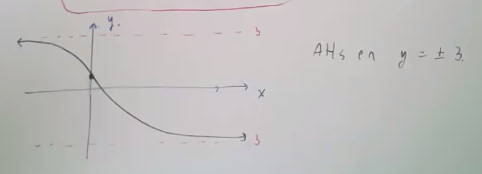
\includegraphics[width=0.8\textwidth]{./Figs/2021-01-18-10-58-09.png}
           % 	\caption{}
           \end{figure}
        \end{center}
    
    \item Integre: $\displaystyle \int \frac{y-2}{y^2-9}$ 
        \begin{center}
           \begin{align*}
               \frac{y-2}{(y-3)(y+3)} = \frac{A}{y-3} + \frac{B}{y+3} \\ 
               y-2 = A(y+3)+B(y-3) \\ 
                y=3: \qq  1 = 6A \qimplies A = 1/6 \\ 
                y =-3: \qq -5 = -6B \qimplies B = 5/6 \\ 
                \frac{A}{y-3} + \frac{B}{y+3} = \frac{1}{6}\ln\p{ y-3 } + \frac{5}{6}\ln\p{ y+3 } +c \\  
                \text{ La ED } \qq  \frac{d y}{d x} =y^2-9 \qimplies y^2-9=0 \qq \text{ cuando: } \qq y \pm 3 \\ 
                \text{ Tiene otras dos soluciones $y = \pm 3$ contantes.} \\ 
                \text{ Solución general:  } \qq y = 3(1+e^{6x+6c}) \\ 
                \text{ Las soluciones $y\pm 3$ se conocen como soluciones singulares: } \\ 
                \text{ Porque:  } \qq \int \frac{dy}{y^2-9} \qq \text{ se indefine en  } \qq x\pm 3 \\ 
           \end{align*}
        \end{center}
\end{enumerate}

Solución singular:
\begin{itemize}
    \item La ED $\displaystyle \frac{dy}{dx}=g(x)h(y)$  tiene soluciones cuando $h(y)=0$.
    \item Solución singular de una ED: son las soluciones $y=c$  donde $h(c)$ 
\end{itemize}
